\section{Software \& Code Implementation}

This section describes the software developed for the Bako OBD ISS platform, covering the embedded firmware running on the ESP32 microcontroller, the battery management decoding logic, the cloud publishing pipeline, and the validation strategy used to verify correct behavior at each layer.

% ─────────────────────────────────────────────────────────────────────────────
\subsection{Firmware Architecture \& RTOS Integration}

The ESP32 firmware is built on the \textbf{Arduino framework} using the \textbf{PlatformIO} build system~\cite{platformio}, which provides dependency management, cross-compilation, and serial monitoring in a single toolchain. Although the Arduino framework does not expose the underlying FreeRTOS scheduler directly, the ESP32's dual-core architecture is leveraged implicitly: the Arduino \texttt{loop()} function executes on Core 1 while the Wi-Fi/Bluetooth stack occupies Core 0. All BMS-related tasks — CAN frame reception, state accumulation, and HTTP publishing — run sequentially on Core 1 without preemption, which simplifies state management and eliminates the need for mutexes at the firmware level.

The firmware follows a \textbf{cooperative, interrupt-driven} model. The MCP2515 CAN transceiver asserts an active-low \texttt{INT} line (GPIO 4) each time a new frame is placed in its receive buffer. The main loop polls this pin continuously and drains all pending frames before entering the timed publish cycle. This design ensures that no CAN frame is ever dropped due to buffer overflow, even during the longer HTTP transaction window.

The overall execution model is summarized in Figure~\ref{fig:fw-flow}.

\begin{figure}[H]
    \centering
    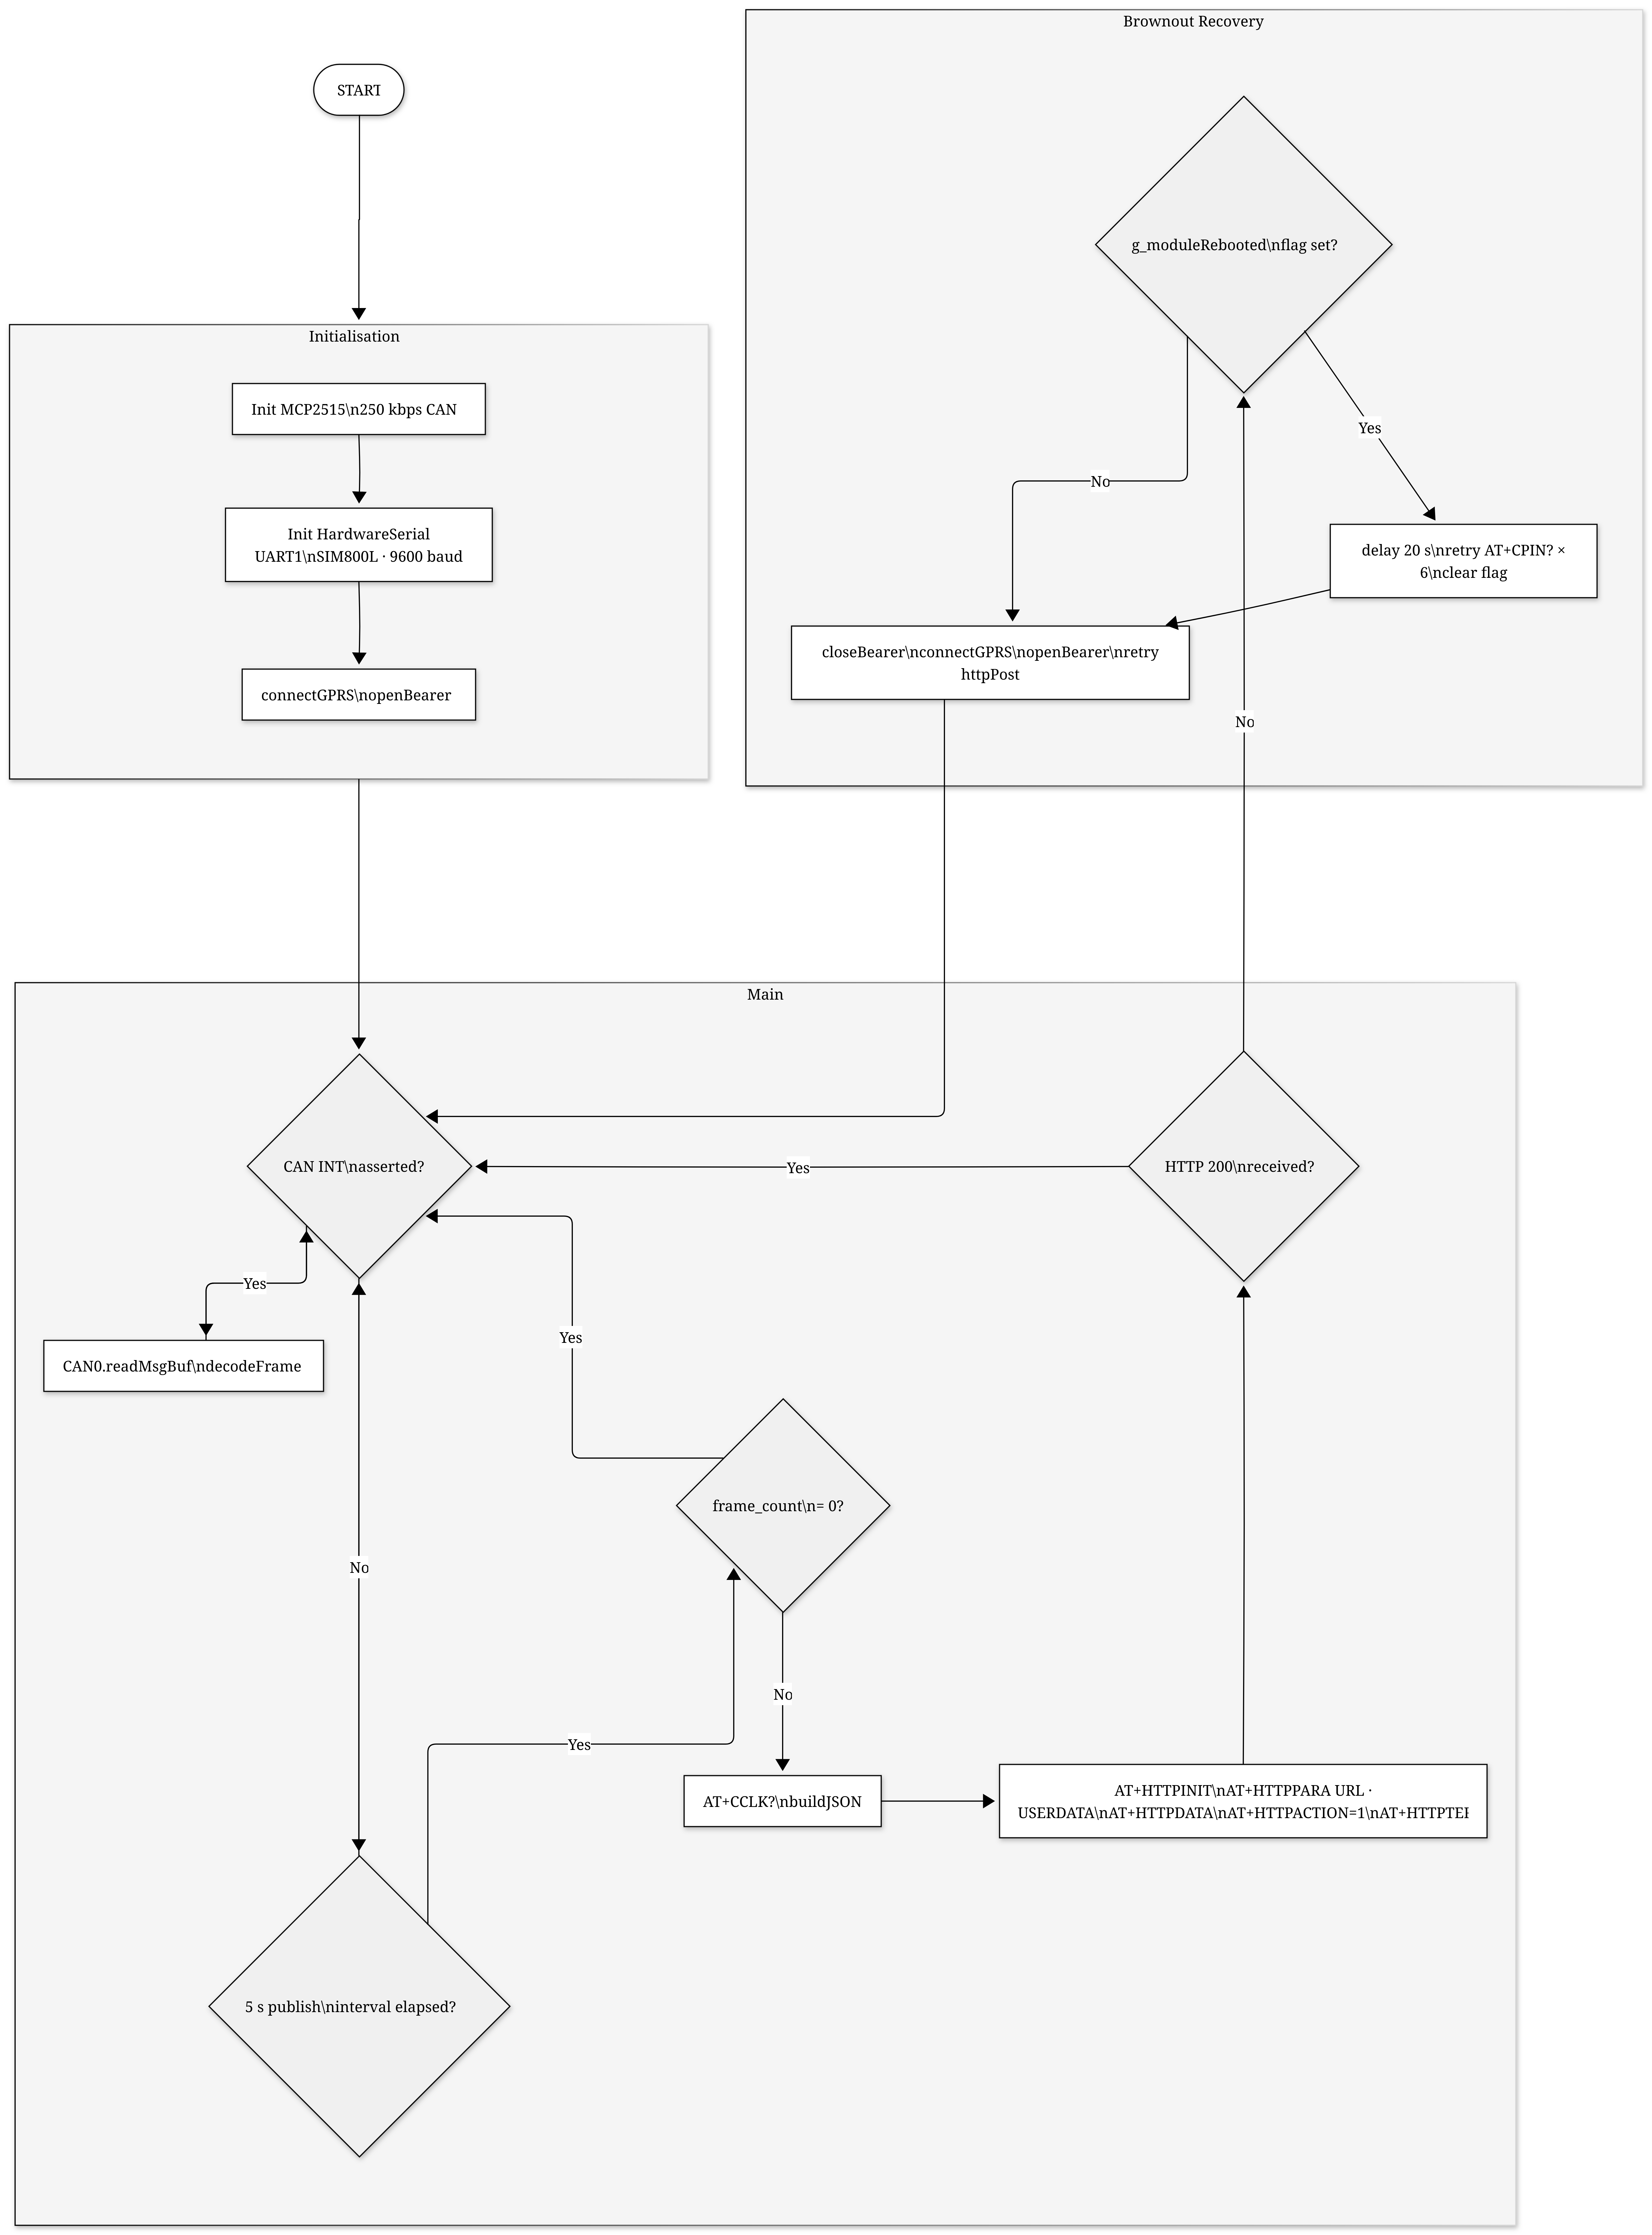
\includegraphics[width=0.7\textwidth]{images/firmware-flow-s.png}
    \caption{Firmware main-loop execution model: CAN drain $\rightarrow$ publish every 5 s}
    \label{fig:fw-flow}
\end{figure}

The SIM800L GPRS module (driven via the SIM800L AT command protocol) is connected to \textbf{HardwareSerial UART1} (GPIO 16/17) at 9600 baud. HardwareSerial was chosen over SoftwareSerial because the module's AT+HTTP* responses can arrive as multi-line bursts that SoftwareSerial's byte-at-a-time interrupt handler occasionally corrupts at 9600 baud on a loaded CPU.

% ─────────────────────────────────────────────────────────────────────────────
\subsection{BMS Firmware}
\label{sec:bms-firmware}

The BMS firmware is responsible for reading raw CAN frames from the O'CELL IFS60.8-500-F-E3 battery management system~\cite{ocellspec}, decoding them according to the \textbf{SAE J1939} standard~\cite{bakocan}, maintaining a live BMS state structure, and serializing that state to JSON for cloud upload.

\subsubsection{CAN Bus Interface}

The physical CAN interface uses a \textbf{MCP2515} controller connected to the ESP32 via the VSPI bus at 10 MHz. The bus operates at \textbf{250 kbps}, which is the standard J1939 baud rate for vehicle control networks~\cite{saej1939}. All frames from the O'CELL BMS use 29-bit extended CAN identifiers, formatted according to the J1939 Parameter Group Number (PGN) convention:

\begin{equation}
    \label{eq:j1939-id}
    \text{CAN ID} = 0x18\_\text{FUNC}\_\text{SUB}\_\text{SA}
\end{equation}

where \texttt{FUNC} is the PGN function byte that identifies the frame type, \texttt{SUB} encodes sub-addressing or destination, and \texttt{SA} = 0xF4 is the source address of the BMS module.

The MCP2515 library is configured in \texttt{MCP\_ANY} mask mode so that all frames on the bus are received without hardware fiGPRSring. Software-side fiGPRSring is performed in the \texttt{decodeFrame()} function by inspecting the \texttt{FUNC} and \texttt{SUB} bytes extracted from the 29-bit ID.

\subsubsection{Supported Frame Types}

Five distinct frame types are decoded, covering all BMS data needed for monitoring and fault diagnosis. Table~\ref{tab:can-frames} lists each frame with its CAN ID, transmission rate, and data content.

\begin{table}[h]
    \centering
    \caption{O'CELL BMS CAN Frame Map (SAE J1939, 250 kbps)}
    \label{tab:can-frames}
    \begin{tabular}{llcl}
        \toprule
        \textbf{CAN ID} & \textbf{Name} & \textbf{Rate (ms)} & \textbf{Content} \\
        \midrule
        \texttt{0x18C8--CC28F4} & Cell voltages (5 frames) & 500 & 4 cells each, big-endian uint16, 1 mV/bit \\
        \texttt{0x18B428F4}     & Temperature probes        & 500 & Up to 8 probes, raw $-$ 40 = °C \\
        \texttt{0x18FF28F4}     & BMS Basic Message 1       & 100 & SOC, current, voltage, fault flags \\
        \texttt{0x18FE28F4}     & BMS Basic Message 2       & 100 & Min/max cell mV, discharge limit \\
        \texttt{0x18FFE5F4}     & Charging request          & 500 & Max charge V, max charge A, start signal \\
        \bottomrule
    \end{tabular}
\end{table}

\paragraph{Cell Voltage Frames (0x18C8--CC28F4).}
The 19 battery cells are transmitted across five consecutive frames. Each frame carries four cells encoded as big-endian 16-bit unsigned integers, with a resolution of 1 mV per bit. The last frame (0x18CC28F4) covers cells 17--19 and pads the unused fourth slot with 0x0000. The firmware detects and skips zero-padded slots:

\begin{verbatim}
for (int i = 0; i < 4; i++) {
    uint16_t mv = u16be(data, i * 2);
    if (mv != 0 && (base + i) < 19)
        bms.cell_mv[base + i] = mv;
}
\end{verbatim}

After each group update, aggregate statistics (minimum, maximum, average) are recomputed from all non-zero cells, and a voltage-based SOC estimate is derived as described in Section~\ref{sec:soc-cal}.

\paragraph{BMS Basic Message 1 (0x18FF28F4).}
This 100 ms frame carries the core operational state of the pack. The byte layout is as follows:

\begin{itemize}
    \item \textbf{Byte 0} — Status bit-field: charge cable connected (bit 0), charging in progress (bit 1), discharging in progress (bit 2), BMS ready (bit 3), discharge contactor closed (bit 4), charge contactor closed (bit 5).
    \item \textbf{Byte 1} — State of charge from the BMS coulomb counter (0--100\%).
    \item \textbf{Bytes 2--3} — Pack current as a little-endian uint16 with a $-$5000 offset and 0.1 A/bit scaling. Positive values indicate discharge; negative values indicate charging.
    \item \textbf{Bytes 4--5} — Direct BMS pack voltage, little-endian uint16, 0.1 V/bit.
    \item \textbf{Byte 6} — Fault severity level (0 = normal, 1 = serious fault).
    \item \textbf{Byte 7} — Fault code (see Table~\ref{tab:fault-codes}).
\end{itemize}

\begin{table}[h]
    \centering
    \caption{BMS Fault Code Map (byte 7 of 0x18FF28F4)}
    \label{tab:fault-codes}
    \begin{tabular}{cl}
        \toprule
        \textbf{Code} & \textbf{Description} \\
        \midrule
        0x00 & No fault (normal operation) \\
        0x01 & Over-temperature — severe \\
        0x02 & Total pack voltage too high \\
        0x03 & Total pack voltage too low \\
        0x04 & Discharge over-current \\
        0x05 & Cell voltage too high \\
        0x06 & Cell voltage too low \\
        \bottomrule
    \end{tabular}
\end{table}

\paragraph{Temperature Probes (0x18B428F4).}
Up to eight thermal probes are encoded as single bytes using the formula $T[\text{°C}] = \text{raw} - 40$~\cite{ds18b20datasheet}. A raw value of 0xFF indicates a disconnected sensor and is skipped. The O'CELL pack fitted to the vehicle contains four active probes.

\paragraph{Charging Request (0x18FFE5F4).}
This frame is transmitted by the BMS toward the on-board charger. It specifies the maximum allowable terminal voltage (bytes 0--1, 0.1 V/bit) and maximum charge current (bytes 2--3, 0.1 A/bit). Bit 0 of byte 4 being clear signals that the BMS is requesting the charger to begin charging.

\subsubsection{BMS State Structure}

All decoded values are accumulated into a single \texttt{BMSData} struct that persists across frames and represents the most recent complete snapshot of the battery's state. The struct is updated in-place by \texttt{decodeFrame()} and read atomically by \texttt{buildJSON()} at each publish cycle. Because the firmware runs single-threaded, no locking is required.

\subsubsection{SOC Calibration}
\label{sec:soc-cal}

The firmware uses a \textbf{voltage-based SOC estimate} derived from the average cell voltage~\cite{lifepo4soc}. This method was selected because it correlates closely with the vehicle's own dashboard reading, unlike the BMS internal coulomb counter which can drift over time~\cite{bmssoc}.

The calibration was performed over four separate on-vehicle sessions, comparing the computed average cell voltage with the vehicle's onboard display:

\begin{equation}
    \label{eq:soc}
    \text{SOC} [\%] = \frac{\overline{V}_{\text{cell}} - 2500}{3387 - 2500} \times 100
\end{equation}

where $\overline{V}_{\text{cell}}$ is the average cell voltage in millivolts. The lower bound of 2500 mV/cell corresponds to 0\% SOC (47.50 V pack), and 3387 mV/cell was calibrated to match 100\% on the car display (64.35 V pack). Values above 3387 mV, which occur during active charging, are clamped to 100\%.

Table~\ref{tab:soc-cal} shows the four calibration sessions used to arrive at the 3387 mV reference point.

\begin{table}[h]
    \centering
    \caption{SOC Calibration Data — Four On-Vehicle Sessions}
    \label{tab:soc-cal}
    \begin{tabular}{cccc}
        \toprule
        \textbf{Session} & \textbf{Avg cell (mV)} & \textbf{Car display (\%)} & \textbf{Solved top (mV)} \\
        \midrule
        2026-03-31 10:06 & 3301.6 & 89.0 & 3400.7 \\
        2026-03-31 10:57 & 3306.2 & 89.0 & 3405.8 \\
        2026-04-01 13:03 & 3284.8 & 89.4 & 3377.9 \\
        2026-04-01 16:04 & 3285.0 & 88.4 & 3387.4 \\
        \midrule
        \multicolumn{3}{r}{\textbf{Adopted reference}} & \textbf{3387 mV} \\
        \bottomrule
    \end{tabular}
\end{table}

\subsubsection{Cloud Publishing via SIM800L}

At every 5-second publish interval, the firmware calls \texttt{buildJSON()} to serialize the current \texttt{BMSData} struct into a nested JSON document using the ArduinoJson v7 library~\cite{arduinojson}, then calls \texttt{httpPost()} to deliver it to the VPS backend via SIM800L GPRS.

The payload uses a five-section nested schema: a top-level envelope wraps \texttt{battery}, \texttt{temperatures}, \texttt{solar}, \texttt{dc\_dc}, and \texttt{vehicle} sub-objects. Individual cell voltages are encoded as a 1-based JSON array (\texttt{cells[0] = null}, \texttt{cells[1]\ldots cells[19] = \{mv, status\}}). Temperature probes follow the same convention in \texttt{temperatures.battery\_cells}. Sensors not yet instrumented (solar, DC/DC, vehicle) appear as \texttt{null}-valued fields so the schema remains stable as additional sensors are commissioned.

The HTTP transaction uses the SIM800L's native \textbf{AT+HTTP*} command set over plain HTTP (AT+HTTPSSL=0). The sequence is:

\begin{enumerate}
    \item \texttt{AT+HTTPTERM} — close any stale session from a previous transaction.
    \item \texttt{AT+HTTPINIT} — open a new HTTP session.
    \item \texttt{AT+HTTPPARA="URL",...} — set the full endpoint URL.
    \item \texttt{AT+HTTPPARA="USERDATA","X-Api-Key: \textit{key}\textbackslash r\textbackslash n"} — inject the API authentication header.
    \item \texttt{AT+HTTPDATA=\textit{len},10000} — upload the JSON body.
    \item \texttt{AT+HTTPACTION=1} — execute the HTTP POST and wait for \texttt{+HTTPACTION:} response.
    \item \texttt{AT+HTTPTERM} — close the session.
\end{enumerate}

During the AT+HTTPACTION wait loop (up to 30 s), the firmware continues draining CAN frames from the MCP2515 receive buffer so that no BMS data is lost while the module is busy.

\subsubsection{Brownout Recovery}

A known failure mode of the SIM800L is a mid-transaction power brownout caused by the $\sim$1.5 A peak current during GPRS transmission exceeding the supply rail's transient capability. When this occurs, the module resets and emits an unsolicited \texttt{"Call Ready"} string in its UART output.

The firmware detects this string in all three response handlers: \texttt{sendAT()}, \texttt{sendATExpect()}, and the \texttt{HTTPACTION} wait loop and sets a global \texttt{g\_moduleRebooted} flag. When a publish cycle fails and this flag is set, the recovery sequence is:

\begin{enumerate}
    \item Wait 20 s for the SIM card and GPRS stack to re-initialize.
    \item Retry \texttt{AT+CPIN?} up to six times at 4-second intervals.
    \item Re-open the GPRS bearer and retry the publish once more.
\end{enumerate}

The hardware fix is to add a 2200~\textmu{}F / 6.3~V bulk capacitor close to the module VBAT pin, as incorporated into PCB Revision RECTIFICATION\_2.

% ─────────────────────────────────────────────────────────────────────────────
\subsection{CAN Frame Parser}
\label{sec:can-frame-parser}

The \texttt{parse\_can()} function in the Python backend implements the BAKO CAN Protocol Rev~1.0, decoding all frames broadcast by the BMS (SA = 0xF4) and all sensor gateway frames transmitted by the ESP32 (SA = 0xAA). A companion \texttt{parse\_sensor()} function handles the \texttt{SENSOR:} text-line fallback format emitted by the Python simulator.

\subsubsection{BMS Frames (SA = 0xF4)}

Table~\ref{tab:can-parser-bms} lists all five BMS frame types decoded by \texttt{parse\_can()}, with their CAN IDs, transmission cycles, decoded fields, and key decoding logic.

\begin{table}[H]
\centering
\caption{BMS CAN Frame Parser --- SA = 0xF4 (O'CELL BMS)}
\label{tab:can-parser-bms}
\small
\begin{tabular}{>{\ttfamily}p{3.5cm} c p{4.5cm} p{4.0cm}}
\toprule
\textbf{CAN ID} & \textbf{Cycle} & \textbf{Fields decoded} & \textbf{Key decoding logic} \\
\midrule
0x18FF28F4 & 100 ms & SOC\%, pack current, pack voltage, fault level, error code & Pack current: (uint16\_LE $-$ 5000) $\times$ 0.1~A; Pack voltage: uint16\_LE $\times$ 0.1~V \\
\midrule
0x18FE28F4 & 100 ms & Max/min cell voltage, max/min temp, max discharge current & Temperatures: uint8 $-$ 40~°C; 0xFF = not connected \\
\midrule
0x18C8--CC28F4 & 500 ms & All 19 cell voltages (4 per frame) & Big-endian uint16 mV pairs; PF byte determines group index (0xC8 = group 0 $\rightarrow$ cells 1--4) \\
\midrule
0x18B428F4 & 500 ms & Up to 8 temperature probe values & uint8 offset $-$40~°C; 0xFF = probe not connected \\
\midrule
0x18FFE5F4 & 1000 ms & Max charge voltage, max charge current & uint16\_LE $\times$ 0.1~V / 0.1~A \\
\bottomrule
\end{tabular}
\end{table}

\subsubsection{ESP32 Sensor Gateway Frames (SA = 0xAA)}

In addition to receiving BMS frames, the ESP32 re-broadcasts external sensor readings as J1939-formatted CAN frames using its own source address (SA = 0xAA). This allows any device on the bus to consume solar, MPPT, thermal, and vehicle state data using a standard CAN interface. Table~\ref{tab:can-parser-esp32} lists all eight gateway frame types.

\begin{table}[H]
\centering
\caption{ESP32 Sensor Gateway CAN Frame Map --- SA = 0xAA}
\label{tab:can-parser-esp32}
\small
\begin{tabular}{>{\ttfamily}p{3.2cm} c p{8.0cm}}
\toprule
\textbf{CAN ID} & \textbf{Cycle} & \textbf{Content} \\
\midrule
0x18D001AA & 200 ms & Solar panel current before MPPT — raw + 5-cycle average (uint16\_LE $\times$ 0.1~A) \\
0x18D101AA & 200 ms & Solar panel voltage + open-circuit $V_{oc}$ (uint16\_LE $\times$ 0.1~V) \\
0x18D201AA & 200 ms & MPPT output current + mode (0=off / 1=track / 2=CV / 3=float) + efficiency~\% \\
0x18D301AA & 200 ms & DC/DC 12~V output voltage ($\times$~0.01~V) + current ($\times$~0.1~A; 0xFFFF = not fitted) \\
0x18D401AA & 1000 ms & Motor temperature (uint8 $-$ 40~°C) \\
0x18D501AA & 1000 ms & MPPT heatsink temperature (uint8 $-$ 40~°C) \\
0x18D601AA & 1000 ms & DC/DC heatsink temperature (uint8 $-$ 40~°C) \\
0x18D701AA & 500 ms & Handbrake position: 0 = released, 1 = engaged, 0xFF = sensor fault; + debounce flag \\
0x18D801AA & 500 ms & GNSS information (position, speed, heading) \\
\bottomrule
\end{tabular}
\end{table}

\subsubsection{SOC Representations and SOH Calculation}

Three distinct SOC representations are maintained simultaneously by the parser:

\begin{description}
    \item[\texttt{soc\_bms}] Raw coulomb-counter value from byte~2 of 0x18FF28F4. Directly reported by the BMS hardware; prone to drift over long charge/discharge cycles.

    \item[\texttt{soc}] Voltage-based SOC derived from the average cell voltage using the calibrated formula (Equation~\ref{eq:soc}):
    \[
        \text{SOC} = \frac{\overline{V}_{\text{cell}} - 2500}{3387 - 2500} \times 100, \quad \text{clamped to } [0, 100]\%
    \]
    The upper reference (3387~mV) was calibrated from four real vehicle logs. This is the primary value displayed on the dashboard.

    \item[\texttt{soc\_coulomb}] Charge request signal derived from 0x18FFE5F4 (the charging request frame), used for charger control decisions. The frame carries the BMS-requested maximum charge voltage and current; its \texttt{start\_signal} bit is monitored to track active charging state.
\end{description}

State of Health (SoH) is calculated from the ratio of the measured actual capacity to the rated pack capacity:
\[
    \text{SoH} = \frac{C_{\text{actual}}}{C_{\text{rated}}} \times 100 = \frac{44.7}{50.0} \times 100 = 89.4\%
\]

% ─────────────────────────────────────────────────────────────────────────────
\subsection{Motor Control Algorithms}

Motor control algorithms are outside the scope of this monitoring system. The ESP32 firmware reads and monitors motor-related sensor data --- specifically motor temperature via DS18B20 and current draw via the ACS712/ACS758 sensors --- but does not interface with the motor controller or implement any drive control logic. Motor speed and torque management remain the responsibility of the existing vehicle control electronics. This boundary is intentional: the monitoring system observes and reports motor operating conditions without intervening in the drivetrain control loop.

% ─────────────────────────────────────────────────────────────────────────────
\subsection{Vehicle Management Unit (VMU) Software}

The Vehicle Management Unit (VMU) is implemented on the same ESP32 microcontroller and is responsible for the higher-level coordination layer above raw sensor acquisition. Specifically, the VMU software handles four functions:

\begin{description}
    \item[\textbf{Data aggregation}] Collecting decoded CAN frames from the BMS (cell voltages, SOC, pack current, temperatures, and fault flags) together with readings from external sensors (DC/DC voltage, MPPT current, motor temperature, and handbrake position) into a unified telemetry structure.

    \item[\textbf{Data formatting}] Structuring all acquired telemetry into a consistent JSON schema for transmission to the dashboard over WebSocket or to the cloud back-end via the SIM800L GSM/GPRS module.

    \item[\textbf{Communication management}] Switching between Wi-Fi Access Point mode (for local dashboard access) and Serial mode (for USB-connected debugging and development), based on the firmware build configuration.

    \item[\textbf{Alert handling}] Monitoring configured thresholds --- including over-temperature limits for the motor and DC/DC converter, battery fault flags from the BMS, and handbrake engagement --- and updating the status LED outputs and dashboard warning panels accordingly.
\end{description}

The VMU software does not perform low-level motor control or BMS internal management; it only reads data from those systems and presents it to the operator.

% ─────────────────────────────────────────────────────────────────────────────
\subsection{ESP32 Access Point Mode}

The ESP32 operates in \textbf{Wi-Fi Access Point (AP) mode} for local dashboard access, having been migrated from an earlier Station Mode implementation. The ESP32 chip supports two distinct Wi-Fi operating modes: Station Mode (STA), where it joins an existing router and receives a DHCP-assigned IP; and Access Point Mode (AP), where it becomes the router, broadcasts its own SSID, and assigns addresses to connecting devices with no external router required.

\subsubsection*{Why Station Mode Was Replaced}

The original firmware connected the ESP32 to a home Wi-Fi router as a station. This introduced three practical drawbacks: the SSID and password were hardcoded, so using the system in a different location required reflashing; the router's DHCP server assigned a different IP address after every reboot, requiring firmware updates to match the PC's current address; and without a nearby router, the simulation environment required a mobile hotspot workaround that added extra configuration steps. AP mode resolves all three issues: the ESP32 brings its own network, the IP address 192.168.4.1 never changes, and the system operates in any location without code changes.

\subsubsection*{AP Mode Internal Operation}

When \texttt{WiFi.softAP()} is called, the ESP32 radio switches to infrastructure mode. The built-in DHCP server listens on 192.168.4.1 and issues leases from the pool 192.168.4.2--192.168.4.11. The application code opens a \texttt{WiFiServer} on port 9000. When a client connects to 192.168.4.1:9000, the lwIP stack completes the TCP three-way handshake and places the connection in the accept queue for the firmware to service.

\subsubsection*{Firmware Changes}

The migration from Station to AP mode required minimal changes, isolated entirely to the Wi-Fi and TCP layer. The simulation engine, phase logic, frame encoders, and timing are identical to the station-mode version. The key changes were:

\begin{itemize}
    \item \textbf{Removed:} \texttt{WIFI\_SSID}, \texttt{WIFI\_PASS}, \texttt{SERVER\_IP} constants; \texttt{ensureWiFi()} and \texttt{ensureTCP()} functions.
    \item \textbf{Added:} \texttt{AP\_SSID}, \texttt{AP\_PASS}, \texttt{AP\_CHANNEL} constants; \texttt{WiFiServer server(TCP\_PORT)} global; \texttt{startAP()} and \texttt{ensureClient()} functions.
    \item \texttt{setup()} now calls \texttt{startAP()} and \texttt{server.begin()} instead of \texttt{ensureWiFi()} and \texttt{ensureTCP()}.
    \item \texttt{loop()} calls \texttt{ensureClient()} with a 50~ms yield when no client is connected, keeping the DHCP and beacon tasks running without burning CPU.
\end{itemize}

The \texttt{server.py} dashboard application required zero modifications. It accepts connections on any local interface, including the 192.168.4.x interface created when the PC joins the BAKO\_SMU network. The only operational change for the user is connecting the PC to the \texttt{BAKO\_BMS} Wi-Fi network before launching the server.

% ─────────────────────────────────────────────────────────────────────────────
\subsection{OTA Firmware Updates \& Web Configuration Portal}
\label{sec:ota}

This section documents the third and final stage of the Wi-Fi connectivity evolution. Following the migration from Station Mode to Access Point (AP) Mode, two complementary features were added: Over-The-Air (OTA) firmware flashing and a browser-based configuration portal. Together they make the system fully maintainable in the field without physical access to the PCB.

\subsubsection*{Development Progression Summary}

The connectivity stack evolved through three clearly defined stages. Table~\ref{tab:wifi-evolution} summarises each stage, its purpose, and the limitation that motivated the next iteration.

\begin{table}[H]
\centering
\caption{Wi-Fi Connectivity Evolution Across Three Development Stages}
\label{tab:wifi-evolution}
\small
\begin{tabular}{c >{\bfseries}p{2.5cm} p{4.5cm} p{4.5cm}}
\toprule
\textbf{Stage} & \textbf{Mode} & \textbf{What was achieved} & \textbf{Limitation that led to next stage} \\
\midrule
1 & Station Mode (STA) & ESP32 joins existing Wi-Fi router. DHCP-assigned IP. Dashboard PC on same LAN. & Router dependency, dynamic IP, hardcoded SSID/password in firmware. \\
\midrule
2 & Access Point Mode (AP) & ESP32 is its own router. Fixed IP 192.168.4.1. No external network needed. & Reflashing still required USB cable. Network parameters hardcoded. \\
\midrule
3 & AP + OTA + Web Config & Wireless firmware flashing from IDE. Browser portal to change all network settings without reflashing. & No further limitation — system is fully field-maintainable. \\
\bottomrule
\end{tabular}
\end{table}

\subsubsection*{Over-The-Air Firmware Update}

The \textbf{ArduinoOTA} library was integrated into the ESP32 firmware to allow wireless firmware flashing directly from the Arduino IDE over the existing AP network. The OTA service runs as a lightweight background handler (\texttt{ArduinoOTA.handle()}) called at every loop iteration alongside the TCP and web servers, adding negligible overhead.

\paragraph{Motivation.}
Once the PCB is mounted inside a vehicle enclosure, accessing the USB port for reflashing is impractical. OTA eliminates this constraint: the technician connects a laptop to the \texttt{BAKO\_BMS} Wi-Fi network, selects the network port in the IDE, and clicks Upload — the new firmware is transmitted wirelessly, verified, and applied.

\paragraph{OTA flashing procedure.}
\begin{enumerate}
    \item Power the ESP32 board (vehicle on, or bench supply connected).
    \item Connect the laptop to the \texttt{BAKO\_BMS} Wi-Fi network broadcast by the ESP32.
    \item Open Arduino IDE → Tools → Port. A network port labelled with the OTA hostname (\texttt{BAKO\_OTA} by default) appears automatically.
    \item Select that port, compile, and click \textbf{Upload} as normal.
    \item The IDE transmits the binary wirelessly. The ESP32 verifies integrity and reboots into the new firmware.
\end{enumerate}

\paragraph{Security.}
The OTA service is password-protected to prevent unauthorised firmware injection. The password is configurable through the web portal and stored in NVS flash so it survives reboots. If an active TCP dashboard client is connected when an OTA session begins, the client socket is cleanly closed before flashing starts to prevent data corruption.

\subsubsection*{Web Configuration Portal}

To avoid hardcoding network parameters into the firmware — which would require a reflash every time the AP name, channel, TCP port, or OTA credentials needed changing — a browser-based configuration portal was implemented and served directly by the ESP32 on port~80 using the \textbf{WebServer} library.

The portal is accessible at \texttt{http://192.168.4.1} from any device connected to the ESP32's AP network. It is styled with the BAKO green colour scheme and renders correctly on both desktop browsers and mobile devices.

\begin{figure}[H]
    \centering
    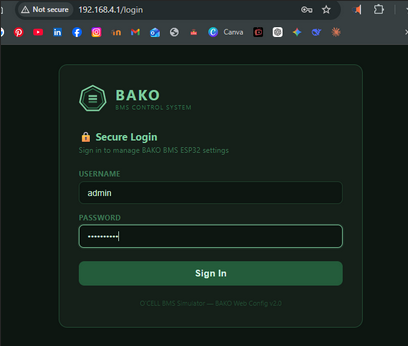
\includegraphics[width=0.55\textwidth]{images/portal-login.png}
    \caption{BAKO BMS web portal login page --- accessible from any browser on the AP network at \texttt{http://192.168.4.1/login}.}
    \label{fig:portal-login}
\end{figure}

After successful login, the operator is directed to the configuration form at \texttt{/config}. Table~\ref{tab:portal-params} lists all configurable parameters.

\begin{table}[H]
\centering
\caption{Configurable Parameters Exposed Through the BAKO Web Portal}
\label{tab:portal-params}
\small
\begin{tabular}{>{\bfseries}p{2.8cm} p{2.5cm} p{7.5cm}}
\toprule
Parameter & Default & Description \\
\midrule
AP SSID        & \texttt{BAKO\_BMS}  & Wi-Fi network name broadcast by the ESP32. \\
AP Password    & \texttt{12345678}   & Minimum 8 characters; leave blank for an open network. \\
WiFi Channel   & \texttt{6}          & Selectable 1--13 to avoid interference with nearby networks. \\
TCP Port       & \texttt{9000}       & Port the Python dashboard server connects to. \\
OTA Hostname   & \texttt{BAKO\_OTA}  & Name visible in Arduino IDE → Tools → Port for OTA flashing. \\
OTA Password   & \texttt{12345678}   & Protects the OTA endpoint against unauthorised firmware injection. \\
\bottomrule
\end{tabular}
\end{table}

\begin{figure}[H]
    \centering
    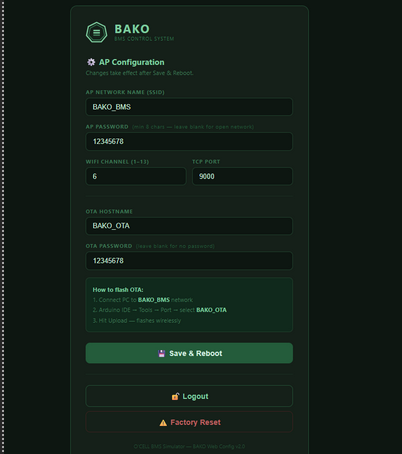
\includegraphics[width=0.55\textwidth]{images/portal-config.png}
    \caption{Web configuration portal --- AP Configuration page showing SSID, password, Wi-Fi channel, TCP port, OTA hostname, and OTA password fields.}
    \label{fig:portal-config}
\end{figure}

\subsubsection*{Web Portal Route Map}

The web server runs on port~80 and handles the following routes. All routes except \texttt{/login} redirect to \texttt{/login} if no valid session cookie is present.

\begin{table}[H]
\centering
\caption{Web Portal Route Map --- All Routes Protected by Session Authentication}
\label{tab:portal-routes}
\small
\begin{tabular}{>{\ttfamily}p{2.8cm} p{2.0cm} p{8.0cm}}
\toprule
\textbf{Route} & \textbf{Method} & \textbf{Function} \\
\midrule
/              & GET        & Redirects to \texttt{/config} if session valid, otherwise to \texttt{/login}. \\
/login         & GET / POST & GET: renders login form. POST: validates credentials; on success sets session cookie and redirects to \texttt{/config}. \\
/config        & GET / POST & GET: renders configuration form (auth required). POST: validates and saves settings, triggers reboot. \\
/logout        & POST       & Invalidates the session token and redirects to \texttt{/login}. \\
/factoryreset  & POST       & Clears all NVS settings and reboots to defaults (auth required). Separate POST-only route prevents accidental GET trigger. \\
\bottomrule
\end{tabular}
\end{table}

\subsubsection*{Simultaneous Services on the ESP32}

After Stage~3 integration, the ESP32 operates four network services concurrently from a single \texttt{loop()} function without measurable impact on CAN frame timing or dashboard refresh rate.

\begin{table}[H]
\centering
\caption{Four Network Services Running Simultaneously on the ESP32 After Stage~3 Integration}
\label{tab:esp32-services}
\small
\begin{tabular}{>{\bfseries}p{3.0cm} p{1.5cm} p{3.0cm} p{5.0cm}}
\toprule
Service & Port & Handler in \texttt{loop()} & Purpose \\
\midrule
Wi-Fi Access Point  & N/A (radio)    & \texttt{WiFi.softAP()} (setup only)  & Broadcasts SSID, runs DHCP, assigns 192.168.4.x addresses. \\
TCP CAN data server & 9000 (default) & \texttt{ensureClient()}               & Streams live CAN frames to the Python dashboard server. \\
OTA update service  & 8266 (mDNS)    & \texttt{ArduinoOTA.handle()}          & Accepts wireless firmware uploads from Arduino IDE. \\
HTTP web config portal & 80          & \texttt{webServer.handleClient()}     & Serves login \& config pages for changing all network settings. \\
\bottomrule
\end{tabular}
\end{table}

% ─────────────────────────────────────────────────────────────────────────────
\subsection{Unit \& Integration Testing}

Software testing for the BMS firmware and cloud pipeline was conducted at three levels: unit testing of the decoding logic, integration testing of the full CAN-to-cloud pipeline, and functional testing of the live dashboard.

\subsubsection{Unit Testing — Frame Decoder}

Each frame type in \texttt{decodeFrame()} was verified by replaying known raw bytes and checking the decoded output against hand-computed expected values. The test case below illustrates verification of cell voltage frame 0x18CB28F4:

\begin{verbatim}
Frame ID: 0x18CB28F4   Data: 0D 3F  0D 38  0D 3A  0D 39

0x0D3F = 3391 mV  -> Cell 13   (big-endian, group = 0xCB - 0xC8 = 3)
0x0D38 = 3384 mV  -> Cell 14
0x0D3A = 3386 mV  -> Cell 15
0x0D39 = 3385 mV  -> Cell 16
\end{verbatim}

Similarly, the signed current decoding formula (offset $-$5000, scale 0.1 A/bit) and the SOC formula (Equation~\eqref{eq:soc}) were verified against values from the real car log file \texttt{bms\_log\_2026-03-10T10-20-02.txt}, which contains 3197 frames captured during an on-vehicle session.

\subsubsection{Integration Testing — Cloud Pipeline}

The end-to-end pipeline was tested without live hardware using the \texttt{replay\_to\_cloud.py} tool, which parses the captured CAN log and replays decoded JSON snapshots to \texttt{POST /api/ingest} at configurable speed. This allowed the following verifications:

\begin{itemize}
    \item The \texttt{/api/ingest} endpoint correctly rejects requests with an invalid \texttt{X-Api-Key} header (HTTP 401).
    \item Each accepted snapshot is stored in the SQLite \texttt{bms\_cloud.db} database with correct timestamp and device ID.
    \item The \texttt{/ws/cloud} WebSocket pushes the most recent snapshot to all connected browser clients within 2 seconds of ingestion.
    \item The \texttt{/api/history} endpoint returns records newest-first with correct JSON structure.
\end{itemize}

\subsubsection{Functional Testing — Live Dashboard}

The live dashboard (\texttt{frontend/index.html}) was tested in both SERIAL and CLOUD modes:

\begin{description}
    \item[SERIAL mode] ESP32 connected via USB to a development laptop. The server decoded incoming frames in real time and the 19-cell voltage grid, SOC ring, and temperature bars updated at 10 Hz without visible lag.
    \item[CLOUD mode] Data replayed from the log file through \texttt{/api/ingest}. The dashboard received snapshots via \texttt{/ws/cloud} at 2 Hz and all panels rendered correctly, including the cloud communication log panel which displayed timestamped RECV and WS events.
    \item[Reconnect behavior] The backend was deliberately stopped while the dashboard was open. The browser WebSocket closed, the connection status indicator turned red (Disconnected), and the overlay appeared. On server restart, the client automatically reconnected within 5 seconds and resumed live updates.
\end{description}

% ─────────────────────────────────────────────────────────────────────────────
\subsection{Web Dashboard}

The BAKO DIAGNOSTICS web dashboard is a dark-theme, single-page web application that provides a real-time overview of the entire vehicle monitoring state. It is served by the FastAPI back-end at the root URL (\texttt{/}) and communicates with the server via WebSocket (\texttt{/ws} in serial mode, \texttt{/ws/cloud} in cloud mode). The dashboard requires no installation; any browser that connects to the server IP receives the complete HTML, CSS, and JavaScript in a single response.

\begin{figure}[H]
    \centering
    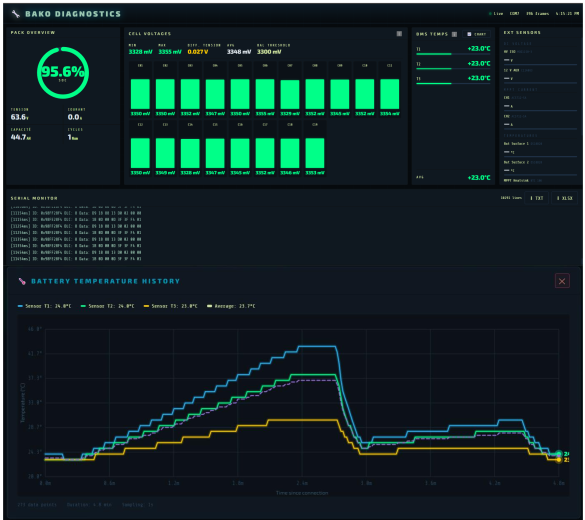
\includegraphics[width=\textwidth]{images/dashboard-screenshot.png}
    \caption{BAKO DIAGNOSTICS live dashboard --- dark-theme single-page interface showing SOC ring gauge, 19-cell voltage grid, temperature time-series chart, and external sensor panel.}
    \label{fig:dashboard-screenshot}
\end{figure}

\subsubsection*{Panel Layout}

The dashboard is organised into four panels arranged to give the engineer an at-a-glance view of all monitored subsystems. Table~\ref{tab:dashboard-panels} describes the content of each panel.

\begin{table}[H]
\centering
\caption{Dashboard Panel Layout}
\label{tab:dashboard-panels}
\small
\begin{tabular}{>{\bfseries}p{3.2cm} p{10.0cm}}
\toprule
Panel & Content \\
\midrule
Left panel &
  State of charge large ring gauge (colour-coded: green $>$30\%, orange 15--30\%, red $<$15\%); pack voltage (V); pack current (A, signed); remaining capacity (Ah); State of Health (SoH) indicator. \\
\midrule
Central panel &
  Individual cell voltage bars for all 19 cells with per-cell colour coding (overvoltage / full / balanced / nominal / low / undervoltage); minimum, maximum, and average cell voltage; cell spread indicator (max $-$ min, mV). \\
\midrule
Temperature panel &
  Four BMS internal temperature probe readings with individual bars; rolling average value; high-temperature threshold alert line. \\
\midrule
Temperature chart &
  Time-series line chart displaying the four individual probe temperatures and their rolling average scrolling in real time. \\
\midrule
Right panel &
  Extended sensor readings: solar panel voltage and current, MPPT output current, MPPT mode and efficiency, DC/DC 12~V output, motor temperature, MPPT heatsink temperature, handbrake status. \\
\midrule
Serial monitor &
  Live scrolling log of raw CAN frames and \texttt{SENSOR:} lines as received from the ESP32. \\
\midrule
File export &
  Export full session log as \texttt{.TXT} or \texttt{.XLSX} with timestamp column. \\
\bottomrule
\end{tabular}
\end{table}

\subsubsection*{Threshold Colour Coding}

Cell voltage bars transition through three colour states based on configurable per-cell thresholds: green when the cell is within its normal operating band (2900--3450~mV for LiFePO4), orange when the cell approaches either end of its safe range, and red when a threshold breach is detected. The SOC ring applies the same three-state scheme based on the pack-level SOC percentage. These thresholds are defined as JavaScript constants in \texttt{frontend/index.html} and can be adjusted without modifying the back-end.

\subsubsection*{Data Export}

The dashboard includes a \textbf{Download CSV} button that retrieves the last 100 snapshots from \texttt{/api/history} and writes them to a timestamped \texttt{.csv} file. The export covers all 19 cell voltages, all four temperature probes, pack SOC, pack voltage, pack current, and extended sensor readings in a single flat row per snapshot, suitable for import into spreadsheet or data analysis tools.

\subsubsection*{Mode Selector}

A mode pill in the dashboard header opens a modal dialog that lets the operator switch the active data source between Serial and Wi-Fi AP modes at runtime, without restarting the server. The mode selection is sent via \texttt{POST /api/mode} and persisted to \texttt{mode\_config.json} so that it is automatically restored on the next server launch.

\begin{itemize}
    \item \textbf{Serial mode} --- auto-detects the connected ESP32 USB port, or accepts manual port entry with a configurable baud rate. The server reads newline-delimited CAN frames from the serial stream.
    \item \textbf{Wi-Fi mode} --- the operator enters the ESP32 IP address (default 192.168.4.1) and TCP port (default 9000), then clicks Apply. The PC must already be connected to the \texttt{BAKO\_BMS} Wi-Fi network.
\end{itemize}

\begin{figure}[H]
    \centering
    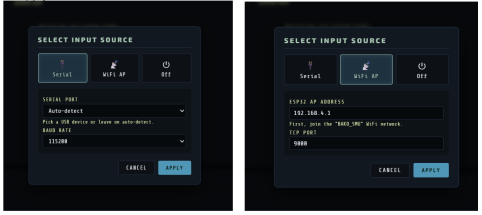
\includegraphics[width=0.85\textwidth]{images/mode-selector.png}
    \caption{Dashboard mode selector dialog: Serial mode (left) and Wi-Fi AP mode (right). Mode is switched without restarting the server.}
    \label{fig:mode-selector}
\end{figure}

% ─────────────────────────────────────────────────────────────────────────────
\subsection{Simulation \& Emulation}

Two complementary simulation tools were developed to enable dashboard testing and firmware validation without requiring a live vehicle or a real O'CELL BMS. Both tools produce data that is indistinguishable from real hardware at the server API level.

\subsubsection*{ESP32 CAN Frame Simulator}

The firmware file \texttt{CAN\_simulation\_7\_phases/CAN\_simulation\_7\_phases.ino} runs on a standalone ESP32 and generates a complete stream of realistic O'CELL BMS CAN frames over USB Serial at 115200 baud, in the same \texttt{[Xms] ID: 0x... DLC: N Data: ...} format that the real vehicle produces.

The simulator models a full charge/discharge lifecycle across seven sequential phases. Table~\ref{tab:sim-phases} describes each phase and its duration.

\begin{table}[H]
\centering
\caption{ESP32 CAN Simulator --- 7-Phase Scenario Cycle}
\label{tab:sim-phases}
\small
\begin{tabular}{c >{\bfseries}p{3.5cm} r p{6.0cm}}
\toprule
Phase & Name & Duration & Description \\
\midrule
0 & REST             & 20~s  & Pack idle at $\approx$72\% SOC; cells balanced; ambient temperature ($\approx$24\textdegree{}C). \\
1 & BULK DISCHARGE   & 120~s & 38~A load; SOC falls 72\%$\to$30\%; temperatures climb; weak cells 7 and 14 develop 15~mV extra sag. \\
2 & LOW SOC WARNING  & 25~s  & BMS throttles current 38~A$\to$12~A; SOC 30\%$\to$18\%; discharge limit ramps down to 15~A. \\
3 & RECOVERY / REST  & 15~s  & Load removed; voltage bounce-back; temperatures plateau. \\
4 & CC CHARGE        & 90~s  & 22~A constant-current charge; SOC climbs 18\%$\to$80\%; cells re-balance. \\
5 & CV TAPER         & 40~s  & Pack near full; charge current tapers 22~A$\to$2~A; spread narrows. \\
6 & FULL REST        & 20~s  & SOC 100\%; zero charge current; cells balanced ($\leq$8~mV spread); loop restarts. \\
\bottomrule
\end{tabular}
\end{table}

Each of the 19 cells has a fixed personality offset ($-20$~mV to $+12$~mV) so the cell spread is realistic and stable across frames. Cells 7 and 14 carry an additional $-18$~mV offset and a load-proportional extra sag, simulating weak cells that would trigger a threshold alert during heavy discharge. The thermal model tracks three sensors at different positions (centre, end-plate, BMS PCB) with individual heating and cooling rates. All six frame types are emitted every 500~ms: cell voltage groups (0x18C8--CC28F4), temperature (0x18B428F4), Basic Message~1 (0x18FF28F4), Basic Message~2 (0x18FE28F4), and charging request (0x18FFE5F4).

\subsubsection{ESP32 Firmware Simulator \& System Interface}

An ESP32-based firmware simulator and monitoring interface were developed to validate the BAKO system without requiring the physical vehicle during each testing session. The simulator reproduces realistic vehicle behaviour by generating sensor telemetry and transmitting it continuously to the monitoring dashboard through TCP socket communication.

The implemented firmware simulates \textbf{14 configurable sensors}, including solar current and voltage, DC/DC converter measurements, motor and MPPT temperatures, battery state of charge (SOC), handbrake status, BMS temperatures, and GNSS speed data. To improve testing coverage, seven automated operating scenarios were integrated: \textit{Parked Idle}, \textit{Solar Charging}, \textit{Normal Driving}, \textit{Heavy Load}, \textit{Low Battery Warning}, \textit{Overheating}, and \textit{Handbrake Fault}. The active scenario changes automatically every 30 seconds, while telemetry data is generated and transmitted every 500~ms.

In addition to the telemetry simulator, an embedded web server was implemented directly on the ESP32. This interface provides a real-time browser-based control panel allowing live sensor monitoring and dynamic parameter modification during testing sessions. Each sensor can operate in one of three modes: \textbf{automatic scenario mode}, \textbf{fixed manual override mode}, or \textbf{randomised range mode} for advanced validation and fault-injection testing.

\begin{figure}[H]
    \centering
    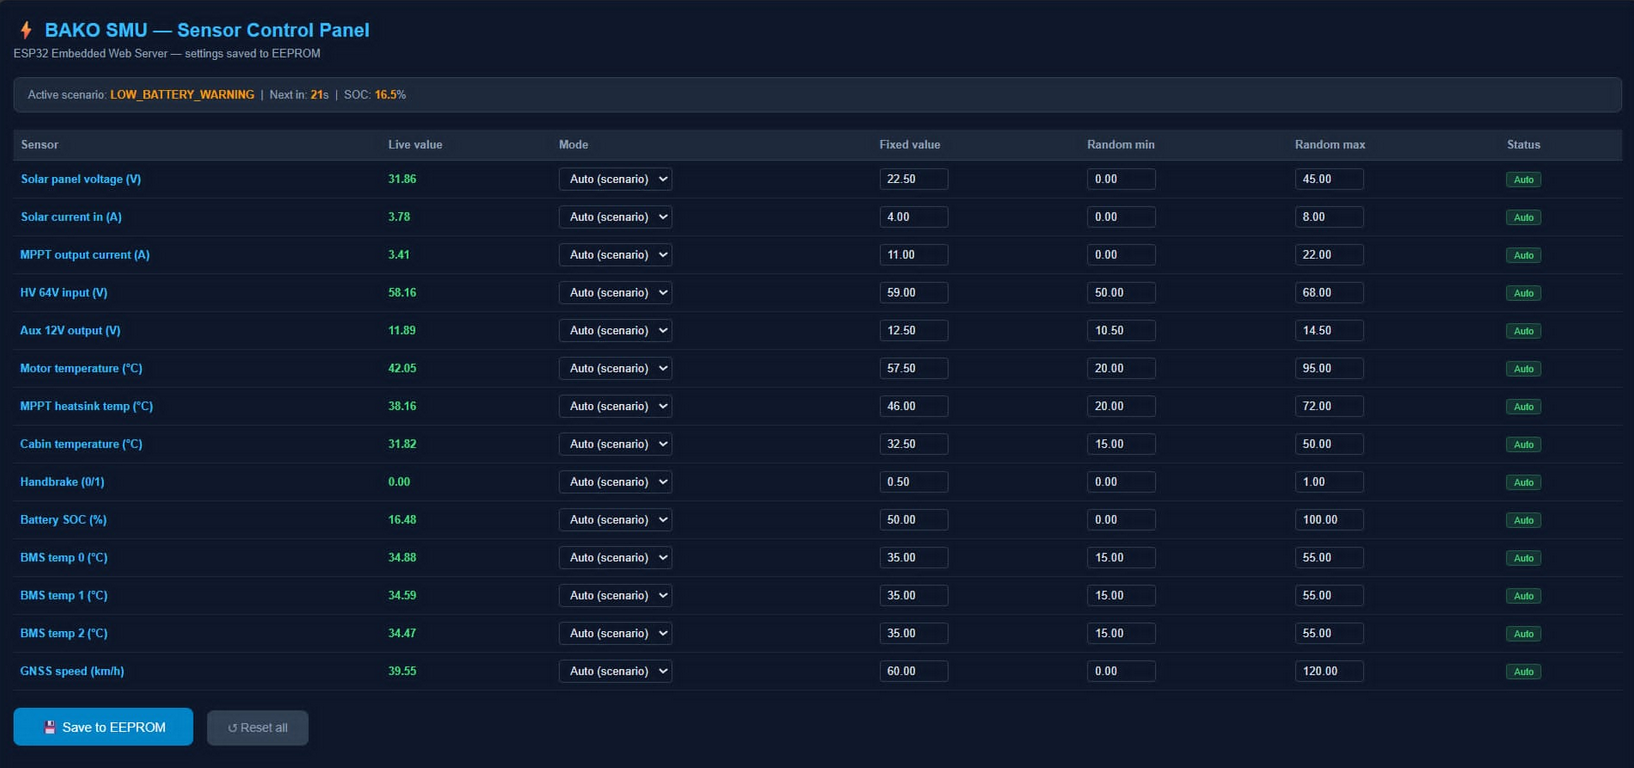
\includegraphics[width=\textwidth]{images/simulator-control-panel.png}
    \caption{BAKO SMU Sensor Control Panel --- browser-based interface served by the ESP32 firmware simulator, showing all 14 sensor channels with live values, scenario mode selectors, and manual override controls.}
    \label{fig:simulator-panel}
\end{figure}

To improve usability and persistence, all sensor configuration parameters are stored locally in \textbf{EEPROM}, allowing settings to remain available after reboot or power cycling. Furthermore, an offline telemetry buffering mechanism was implemented using the ESP32 \textbf{SPIFFS} internal flash filesystem. When the TCP connection becomes unavailable, telemetry data is temporarily stored locally and automatically retransmitted once connectivity is restored.

This testing environment significantly reduces dependency on the physical vehicle during development and debugging phases. It also provides a reproducible and controlled platform for validating embedded communication pipelines, dashboard integration, telemetry visualisation, offline recovery behaviour, and system operation under multiple simulated conditions.

\subsubsection*{Python Log Replay Tool}

The script \texttt{simulate.py} provides a complementary simulation path that uses a captured real-vehicle CAN log rather than synthetic data. It reads the log file \texttt{data/raw/bms\_log\_2026-03-10T10-20-02.txt} (containing 3197 frames from a real on-vehicle session) and pipes it into the live server over a virtual serial port, allowing the full dashboard to operate on authentic data without physical hardware.

The replay sequence is:
\begin{enumerate}
    \item A virtual PTY (pseudo-terminal) pair is created using \texttt{socat}. One end is handed to the server as its serial port; the other is used by the feeder thread to write log lines.
    \item The FastAPI server is launched as a subprocess on port 8787.
    \item Once the server's \texttt{/api/mode} endpoint responds, the script posts \texttt{mode=serial} with the virtual PTY path, switching the server into serial-reader mode.
    \item The browser is opened automatically at \texttt{http://localhost:8787}.
    \item Log frames are streamed to the PTY feeder end with inter-frame delays derived from the original timestamps, scaled by a configurable speed multiplier (default 2$\times$). The log loops continuously until interrupted.
\end{enumerate}

The \texttt{--speed} argument allows accelerated replay (e.g., \texttt{--speed 10} for rapid regression testing) while \texttt{--no-browser} suppresses the automatic browser launch for headless test environments.

\subsubsection{Python Emulator Extension: Local Storage and TCP Transmission}

As an extension to the Python-based sensor emulator, a local storage and TCP communication layer was implemented to improve telemetry reliability and prepare the emulator for remote server integration.

The emulator first generates realistic values for the 14 external sensors, including current, voltage, temperature, handbrake state, and GNSS data. Each generated record is then stored locally in a SQLite database before any transmission attempt. This ensures that telemetry data is preserved even if the network connection is unavailable.

A TCP socket client was also developed to transmit unsent records to a remote server. During local testing, a simulated TCP server was used to reproduce the behaviour of the future VPS server. When the server is available, the client sends the stored telemetry records and marks them as sent in the local database. If the connection fails, the data remains stored locally and is retried automatically during the next transmission cycle.

This architecture implements a \textbf{store-and-forward} mechanism. It allows the emulator to continue operating during internet outages while preventing telemetry loss. Once VPS access is provided, only the server IP address in the TCP client configuration needs to be replaced to enable remote deployment.

The implemented extension therefore adds three key capabilities to the emulator:
\begin{itemize}
    \item local persistence of generated telemetry data using SQLite;
    \item TCP socket transmission instead of WebSocket communication;
    \item offline buffering and automatic retransmission after reconnection.
\end{itemize}

This work prepares the emulator for reliable remote telemetry testing and aligns it with the cloud connectivity objectives of the BAKO monitoring system.

% ─────────────────────────────────────────────────────────────────────────────
\subsection{Wi-Fi Dashboard Connection}
\label{sec:wifi-dashboard}

The \textbf{Wi-Fi dashboard connection} mode allows the FastAPI server to receive telemetry data from the ESP32 over a TCP socket rather than a USB serial port. This mode was implemented to support wireless monitoring sessions where connecting a USB cable to the vehicle is impractical.

\subsubsection*{ReaderManager --- Runtime-Switchable Transport}

The \texttt{ReaderManager} class in \texttt{server\_frame\_parser\_Json.py} owns a single background reader thread and exposes three selectable transport modes:

\begin{description}
    \item[\texttt{serial}] Opens the specified USB/UART serial port (auto-detected or manually specified) and reads newline-delimited CAN frame text.
    \item[\texttt{wifi}] Opens a TCP client socket to the ESP32 AP at the configured IP and port, and reads the same frame format over Wi-Fi.
    \item[\texttt{off}] No reader running; the dashboard displays the ``Disconnected'' state.
\end{description}

Mode selection is persisted to \texttt{mode\_config.json} and restored automatically on the next server launch. When the operator switches mode via the dashboard UI (Section~\ref{fig:mode-selector}), \texttt{ReaderManager} signals the current reader thread to stop (via a \texttt{threading.Event}), waits up to 4~seconds for it to join, then starts the new reader thread with updated configuration.

\subsubsection*{Wi-Fi Reader Loop}

The \texttt{wifi\_reader\_loop()} function implements the TCP client. Its behaviour is:

\begin{enumerate}
    \item Open a \texttt{socket.SOCK\_STREAM} TCP connection to the ESP32 at the configured IP and port (default 192.168.4.1:9000) with a 4-second connection timeout.
    \item On successful connection, set \texttt{state["connected"] = True} and \texttt{state["mode"] = "wifi"} under the shared state lock.
    \item Read the socket in 4096-byte chunks with a 1-second timeout. Split on newline boundaries and pass each complete line to \texttt{process\_line()}, the same CAN-frame parser used in serial mode. A partial final line is buffered until the next chunk arrives.
    \item On any socket error or lost connection, set \texttt{state["connected"] = False}, log the error to \texttt{state["last\_error"]}, wait 2~seconds, and retry the TCP connection. This automatic reconnection handles the case where the ESP32 reboots or moves out of range.
    \item On stop signal, close the socket and exit.
\end{enumerate}

Because the frame format emitted by the ESP32 over Wi-Fi TCP is identical to that emitted over USB Serial, the parsing layer (\texttt{process\_line()}) requires no modification for Wi-Fi mode. The dashboard connection status indicator correctly reflects the Wi-Fi connection state in real time.

% ─────────────────────────────────────────────────────────────────────────────
\subsection{BLE Companion Interface}
\label{sec:ble}

Bluetooth Low Energy (BLE) connectivity was implemented to complement the Wi-Fi dashboard by providing a lightweight, phone-friendly monitoring channel for the vehicle operator. BLE was selected due to its low power consumption, wide smartphone compatibility, and sufficient data throughput for sensor-based telemetry. The ESP32 chip includes a built-in dual-mode Bluetooth radio supporting BLE 4.2 / 5.0, making BLE a zero-hardware-cost addition to the platform.

\subsubsection*{Hardware and Software Platform}

The BLE module runs entirely on the ESP32 development board using the \textbf{NimBLE-Arduino} library, a lightweight and memory-efficient BLE stack well-suited to embedded firmware. Testing was performed using Android BLE scanner applications, including nRF Connect, and a custom Android companion application.

\subsubsection*{GATT Architecture}

The communication follows a GATT (Generic Attribute Profile) client--server model. The ESP32 acts as the \textbf{GATT Server}, exposing a vehicle telemetry service; the Android application acts as the \textbf{GATT Client}, subscribing to and receiving characteristic notifications.

The telemetry service is identified by a project-specific 128-bit base UUID \texttt{12345678-0000-0000-0000-0000000000xx}. Six characteristics are defined, each carrying one real-time sensor stream:

\begin{table}[H]
\centering
\caption{BLE GATT Characteristic Map}
\label{tab:ble-characteristics}
\begin{tabular}{ll}
\toprule
\textbf{Parameter} & \textbf{Characteristic UUID} \\
\midrule
Speed       & \texttt{12345678-0000-0000-0000-000000000001} \\
Voltage     & \texttt{12345678-0000-0000-0000-000000000002} \\
SOC         & \texttt{12345678-0000-0000-0000-000000000003} \\
Current     & \texttt{12345678-0000-0000-0000-000000000004} \\
Temperature & \texttt{12345678-0000-0000-0000-000000000005} \\
RPM         & \texttt{12345678-0000-0000-0000-000000000006} \\
\bottomrule
\end{tabular}
\end{table}

\subsubsection*{ESP32 Implementation}

The BLE stack is initialised in \texttt{setup()} using the NimBLE API:

\begin{enumerate}
    \item \texttt{NimBLEDevice::init()} --- initialises BLE with the device name \textbf{BAKO-Dashboard}, which is broadcast in the advertising packet so that Android devices can discover the ESP32 by name.
    \item \texttt{createServer()} --- creates the GATT server and registers connection callbacks.
    \item \texttt{createService()} --- defines the vehicle telemetry service under its UUID.
    \item \texttt{createCharacteristic()} --- defines each of the six data channels with \texttt{READ | NOTIFY} properties.
    \item \texttt{startAdvertising()} --- makes the device continuously discoverable.
\end{enumerate}

Sensor values are updated every 500~ms in the main loop. Each value is converted to a string and pushed via \texttt{notify()}, which delivers it to any subscribed Android client in real time. Notifications are only sent when a client is connected, avoiding unnecessary radio activity.

\subsubsection*{Connection Handling}

A callback class overrides two methods to manage the BLE connection lifecycle:

\begin{itemize}
    \item \textbf{onConnect} --- triggered when an Android device establishes a connection; suspends advertising to dedicate bandwidth to the active client.
    \item \textbf{onDisconnect} --- automatically restarts advertising so the ESP32 remains discoverable after the client disconnects or moves out of range.
\end{itemize}

This ensures continuous availability without manual reset.

\subsubsection*{Android Integration}

The Android companion application scans for BLE devices by advertised name. After connecting to \textbf{BAKO-Dashboard}:

\begin{enumerate}
    \item The app discovers the GATT telemetry service.
    \item It subscribes to all six characteristics and enables notifications.
    \item Live values (speed, SOC, voltage, current, temperature, RPM) are displayed on a real-time dashboard interface.
\end{enumerate}

\subsubsection*{Coexistence with Wi-Fi}

The ESP32 shares its radio between Wi-Fi and BLE using time-division multiplexing managed by the ESP-IDF coexistence driver. Enabling BLE advertising alongside the Wi-Fi AP increases the Wi-Fi beacon interval slightly but does not affect the cloud GPRS data stream, which runs over the SIM800L UART and is entirely independent of the radio.

\subsubsection*{Challenges Encountered}

\paragraph{Device visibility on Android.}
Initially the ESP32 BLE device did not appear consistently in BLE scanning applications. Investigation revealed that the advertising packet was missing a complete scan response entry for the device name. The issue was resolved by explicitly configuring the NimBLE advertising parameters to include the device name in both the advertising data and the scan response packet, and by ensuring that \texttt{startAdvertising()} is called only after the GATT service is fully initialised.

\paragraph{Apple iOS compatibility.}
Testing on iOS devices proved more restrictive. iOS enforces stricter BLE scanning rules than Android: devices may not appear unless they advertise complete service UUIDs, background scanning is limited, and some characteristics require explicit bonding before they become visible to the application layer. As a result, Android was adopted as the primary testing and deployment platform, where tools such as nRF Connect provide detailed GATT inspection and ease of debugging. iOS support is deferred to a future firmware and app revision.

